\section{Experiments i resultats}
\label{sec:experiments}

% ---------------------------------------------------------------------------------------------------------
\subsection{Dades i preprocessament (exercicis 1-4)}
\label{sec:dades}

El corpus té 4.978 frases d'entrenament, de les quals reservem les 900 últimes per a validació, i 893 de test
(taula~\ref{tab:dades}). Ja en carregar els CSV vam trobar dos problemes. Els camps estan separats per
\texttt{", "} i entre cometes, i si a pandas no se li indica \texttt{skipinitialspace=True}, les cometes es queden
dins del text i apareixen etiquetes que no existeixen, com \texttt{"O}. A més, tot i que l'enunciat parla de BILOU,
el fitxer està en BIO. Vam optar per convertir-lo a BILOU: una \etq{B} aïllada passa a ser \etq{U} i l'última
\etq{I} d'una entitat passa a ser \etq{L}. La conversió es pot desfer i té l'avantatge de marcar explícitament on
acaba cada entitat, però l'hem deixada com a paràmetre per poder comparar els dos esquemes més endavant
(apartat~\ref{sec:extres}).

Com que les frases ja venen tokenitzades i en minúscules, n'hi ha prou de separar per espais, i així es manté una
etiqueta per paraula. El vocabulari es construeix només amb train i les paraules que hi surten un sol cop van a
\etq{<unk>}, perquè altrament el vector de \etq{<unk>} no s'entrenaria mai. El padding té un índex propi que la loss
ignora, i el mateix índex el fem servir per a la quinzena de tokens de validació i test amb etiquetes que no
apareixen a train. Això no amaga cap error: l'avaluació es fa sempre contra les etiquetes originals en text, i
aquests tokens hi compten com a fallades.

\begin{table}[ht]
\centering\small
\caption{Estadístiques del dataset.}
\label{tab:dades}
\begin{tabular}{lr}
\toprule
Frases train / validació / test & 4.078 / 900 / 893 \\
Longitud mitjana (màxima) de les frases & 11,4 (46) paraules \\
Etiquetes BILOU (BIO) & 178 (119) \\
Proporció de tokens \etq{O} & 63,7\% \\
Etiquetes amb un sol exemple a train & 25 \\
Tokens amb etiqueta no vista a train (val / test) & 7 / 10 \\
Vocabulari ($\texttt{min\_freq}=2$) i tokens \etq{<unk>} a test & 589 paraules, 1,44\% \\
\bottomrule
\end{tabular}
\end{table}

% ---------------------------------------------------------------------------------------------------------
\subsection{Model base (exercicis 5-6)}
\label{sec:base}

El model base és senzill: un embedding de 128 dimensions, una LSTM bidireccional de 128 unitats i una capa lineal
que classifica cada token. Abans de passar per la LSTM empaquetem les seqüències amb la seva longitud real, ja que
d'altra manera la direcció cap enrere començaria cada frase llegint desenes de posicions de padding. L'entrenem amb
Adam (LR $10^{-3}$) i aturem l'entrenament quan la F1 d'entitats de validació deixa de millorar.

Aquesta F1, calculada amb seqeval \citep{seqeval} en mode estricte (equivalent a conlleval), és la mètrica de
referència de tot el treball: una entitat només compta com a encertada si en coincideixen el tipus i els límits.
L'accuracy per token, en canvi, diu poca cosa en aquest problema, perquè un model que predigués sempre \etq{O} ja
superaria el 60\%.

\begin{table}[ht]
\centering\small
\caption{Resultats del model base (exercici 6, una llavor).}
\label{tab:base}
\begin{tabular}{lccc}
\toprule
 & F1 entitats & Accuracy token & F1 macro token (sense \etq{O}) \\
\midrule
Validació & 0,975 & 0,989 & 0,820 \\
Test      & 0,953 & 0,977 & 0,707 \\
\bottomrule
\end{tabular}
\end{table}

A test, la F1 micro d'entitats és de 0,95 i la macro, de 0,73 (taula~\ref{tab:base}). La distància entre totes
dues reflecteix el problema principal del dataset: les entitats freqüents, com \etq{fromloc.city\_name}, surten
gairebé perfectes, mentre que moltes de les rares tenen una F1 baixa o directament nul·la. També s'hi veu un primer
indici de sobreajust, ja que la loss de validació arriba al mínim cap a l'època 17 i després puja lleugerament
mentre la de train continua baixant.

% ---------------------------------------------------------------------------------------------------------
\subsection{Metodologia de l'exercici 7}
\label{sec:metodologia}

Per poder comparar variants amb garanties vam escriure un paquet propi (\texttt{ner/}) en què totes
comparteixen el preprocessament, el bucle d'entrenament i l'avaluació, i cada arquitectura és un bloc que es pot
intercanviar. A cada apartat canviem un sol factor respecte al baseline i entrenem cada configuració amb tres
llavors, de manera que a les taules donem la mitjana i la desviació. Les decisions es prenen sempre amb validació;
el test només s'observa. A més de la F1 d'entitats, seguim la F1 macro, el nombre de paràmetres entrenables i el
temps per època. En total han estat 278 entrenaments, unes 3,3 hores en una GPU T4.

Hi ha un detall que cal explicar d'entrada. Per a l'exercici 7 vam afegir a l'aturada un
$\texttt{min\_delta}=0{,}001$, amb la idea d'estalviar èpoques que només milloraven mil·lèsimes, i va resultar
massa estricte: el baseline de l'exercici 7 es queda en 0,946 de test amb cinc llavors, per sota del 0,953 de
l'exercici 6. Com que totes les variants comparteixen el criteri, les comparacions continuen sent vàlides, i a
l'apartat~\ref{sec:final} comprovem que les conclusions es mantenen sense \mindelta.

% ---------------------------------------------------------------------------------------------------------
\subsection{Mida dels embeddings i embeddings preentrenats (7.1)}
\label{sec:emb}

Hem provat embeddings aleatoris de 16 a 512 dimensions i vectors GloVe \citep{glove} de 50, 100, 200 i 300
dimensions, tant congelats com amb \emph{fine-tuning} (figura~\ref{fig:emb}). Dels fitxers de GloVe només hem
guardat els vectors de les paraules que apareixen a ATIS, cosa que dona exactament les mateixes prediccions que
fer servir GloVe sencer (una paraula que no surt mai no es consulta) i no utilitza cap etiqueta de validació ni de
test.

\begin{figure}[ht]
\centering
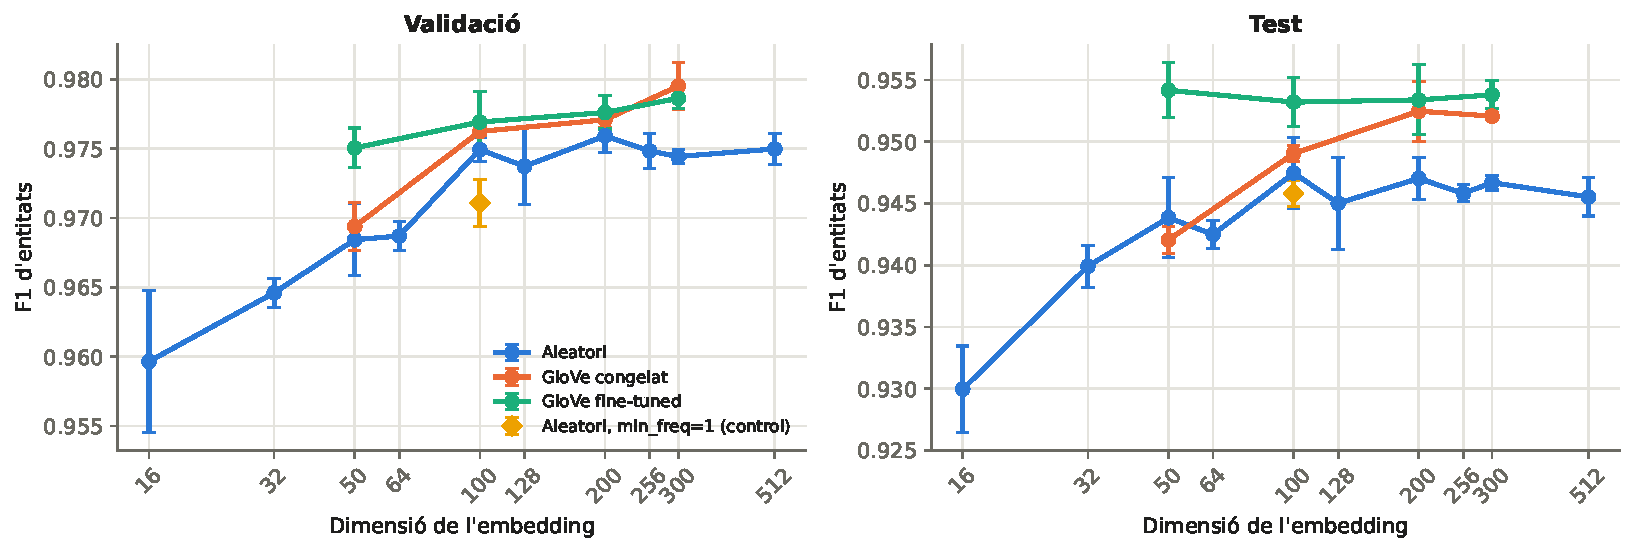
\includegraphics[width=\linewidth]{ex7_1_embeddings}
\caption{F1 d'entitats (mitjana $\pm$ desviació, 3 llavors) segons la dimensió de l'embedding, per a embeddings
aleatoris, GloVe congelat i GloVe \emph{fine-tuned}. El rombe és el control amb $\texttt{min\_freq}=1$.}
\label{fig:emb}
\end{figure}

Amb embeddings aleatoris, la F1 de validació puja de 0,960 amb 16 dimensions a 0,975 amb 100, i a partir d'aquí
pràcticament no es mou. Esperàvem que per sobre de 256 dimensions el model sobreajustés, i no és el que passa.
Els embeddings grans convergeixen més de pressa (la millor època baixa de 25 a 10) i suposem que l'aturada els
talla abans que l'excés de capacitat arribi a fer mal. On sí que es nota una petita pèrdua és en la F1 macro, que
baixa una mica a 300 i 512 dimensions.

GloVe és el canvi més clar de l'apartat. Congelat i amb 300 dimensions arriba a 0,980 de validació, 0,4 punts per
sobre del millor embedding aleatori, i a test tots els GloVe de 100 dimensions o més superen tots els aleatoris.
L'efecte és encara més visible en la F1 macro, que passa de 0,717 al baseline a valors d'entre 0,750 i 0,774, i
això encaixa amb la idea que el que aporta GloVe és coneixement sobre paraules rares. Ara bé, el vocabulari amb
GloVe també inclou les paraules que surten un sol cop a train, i calia descartar que el guany vingués d'aquí. Per
això vam afegir un control amb el vocabulari complet ($\texttt{min\_freq}=1$) i vectors aleatoris, que no millora
(0,971): el guany ve dels vectors. Entre congelar i fer \emph{fine-tuning} no hem trobat una diferència
consistent, i congelar té l'avantatge d'estalviar uns 280.000 paràmetres.

% ---------------------------------------------------------------------------------------------------------
\subsection{Xarxes convolucionals i pooling (7.2)}
\label{sec:cnn}

La convolució l'hem provada de tres maneres (figura~\ref{fig:cnn}): una CNN de paraula davant de la BiLSTM, una
CNN sola i una char-CNN que construeix la representació de cada paraula a partir dels seus caràcters
\citep{mahovy}. El pooling va requerir una mica de reflexió, perquè un \emph{global pooling} redueix tota la frase a
un sol vector i en NER necessitem una sortida per paraula. Finalment l'hem fet servir com a max-pooling local amb
stride 1, com a vector global de la frase concatenat a cada posició i, dins de la char-CNN, sobre els caràcters de
cada paraula.

\begin{figure}[ht]
\centering
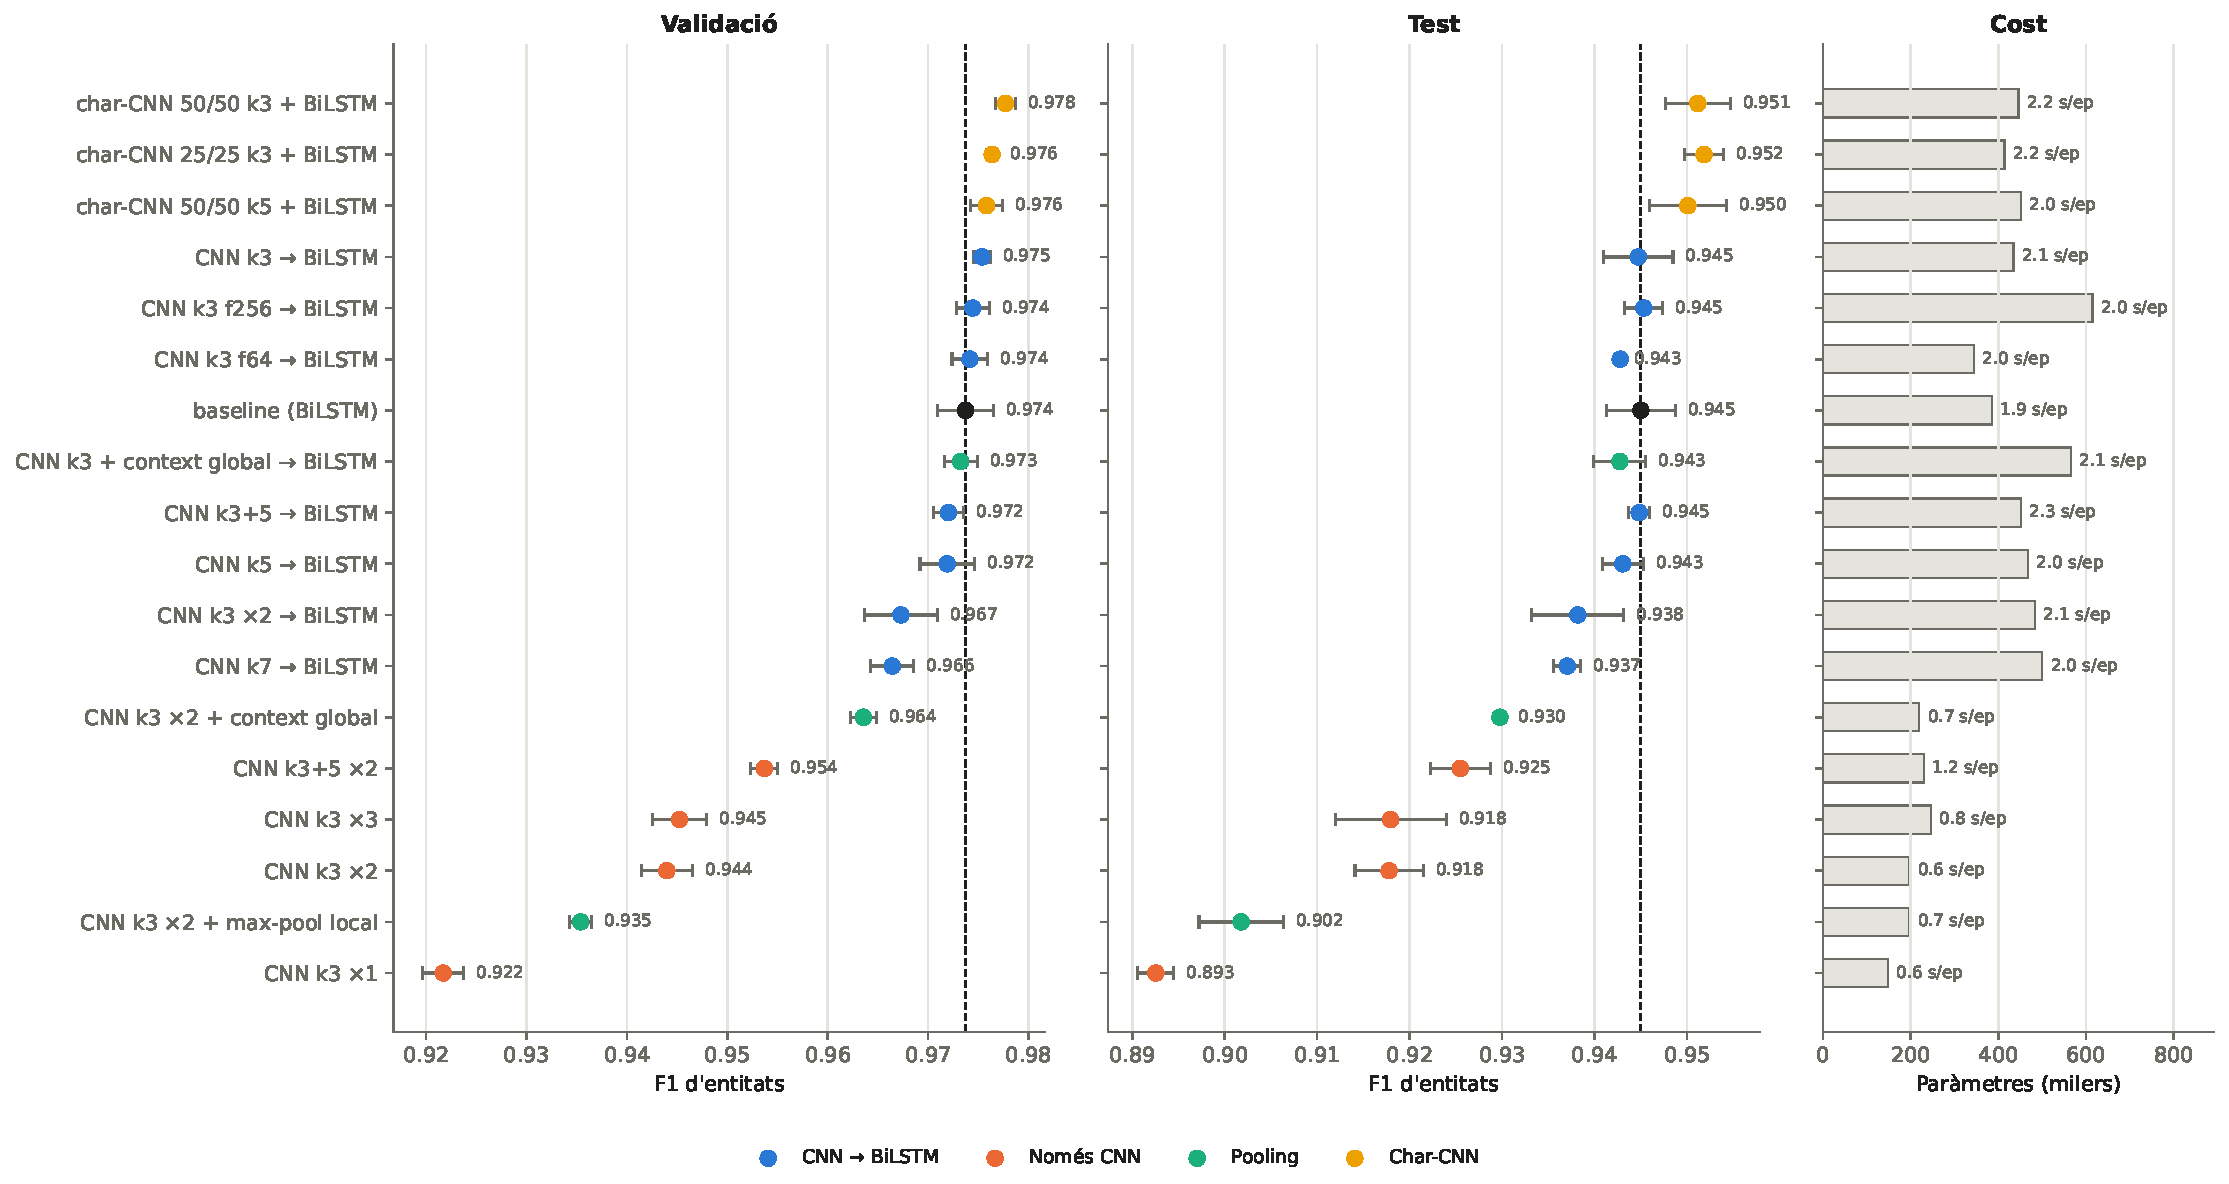
\includegraphics[width=0.9\linewidth]{ex7_2_cnn}
\caption{Variants convolucionals ordenades per F1 de validació: F1 de validació i test (línia discontínua:
baseline) i cost en paràmetres i segons per època.}
\label{fig:cnn}
\end{figure}

Posar una CNN davant de la BiLSTM no ajuda. La millor variant, amb kernel 3, obté 0,975, dins de la variabilitat del
baseline (0,974 $\pm$ 0,003), i els kernels grans o les dues capes fins i tot empitjoren. La nostra lectura és que
la BiLSTM ja recull bé el context local i que la convolució només hi afegeix paràmetres.

Sense recurrència la situació és diferent. La CNN sola queda per sota del baseline, entre 0,92 i 0,95 de
validació, i millora a mesura que creix el camp receptiu: 0,922 amb una capa de kernel 3, 0,944 amb dues i 0,954
combinant kernels de 3 i 5. Té sentit, perquè etiquetes com \etq{arrive\_time} i \etq{depart\_time} depenen de
paraules que poden quedar lluny, fora d'una finestra petita. Per la mateixa raó, el vector de context global és
el que més ajuda a la CNN sola (dos punts de F1 de validació i cinc de F1 macro a test), mentre que sobre la BiLSTM
no aporta res. El max-pooling local, en canvi, empitjora la CNN fins a 0,935, segurament perquè barreja
activacions de paraules veïnes i difumina on comença i on acaba cada entitat.

La char-CNN és l'única variant que supera el baseline més enllà de la variabilitat entre llavors, amb 0,978 de
validació, 0,951 de test i entre 3 i 4 punts més de F1 macro. Pensàvem que l'efecte vindria sobretot de les
paraules desconegudes, però sobre els 76 tokens de test que no surten a train l'accuracy només passa de 0,55 a
0,57-0,60. Creiem, per tant, que la millora ve més aviat de representar bé paraules rares que sí que són al
vocabulari, com números de vol o codis d'aeroport.

% ---------------------------------------------------------------------------------------------------------
\subsection{Xarxes recurrents (7.3)}
\label{sec:rnn}

En aquest apartat hem variat el tipus de cel·la, la direcció, el nombre de capes i la mida de l'estat d'un en un,
i després hem creuat automàticament els valors guanyadors (taula~\ref{tab:rnn}). Per separar l'efecte de la
direcció del de la capacitat hem inclòs també una LSTM unidireccional de 256 unitats, que té la mateixa mida de
sortida que la BiLSTM de 128.

\begin{table}[ht]
\centering\small
\caption{Variants recurrents (3 llavors; la desviació de validació és $\le 0{,}003$ en totes).}
\label{tab:rnn}
\begin{tabular}{lcccr}
\toprule
Configuració & Val F1 & Test F1 & F1 macro test & Paràmetres \\
\midrule
BiLSTM 1$\times$128 (baseline) & 0,9737 & 0,9450 & 0,717 & 386k \\
BiGRU 1$\times$128             & 0,9736 & 0,9494 & 0,724 & 320k \\
LSTM 1$\times$128 (unidir.)    & 0,9475 & 0,9200 & 0,669 & 231k \\
LSTM 1$\times$256 (unidir.)    & 0,9471 & 0,9229 & 0,697 & 517k \\
BiLSTM 2$\times$128            & 0,9738 & 0,9493 & 0,742 & 781k \\
BiLSTM 3$\times$128            & 0,9721 & 0,9428 & 0,710 & 1.176k \\
BiLSTM 1$\times$64             & 0,9747 & 0,9453 & 0,685 & 198k \\
BiLSTM 1$\times$256            & 0,9748 & 0,9494 & 0,738 & 958k \\
BiLSTM 2$\times$256 (creuament) & 0,9765 & 0,9508 & 0,746 & 2.535k \\
\bottomrule
\end{tabular}
\end{table}

El factor que més pesa, amb diferència, és la direcció. Sense context dret la F1 cau 2,6 punts, i la LSTM
unidireccional de 256 unitats no en recupera cap, de manera que el que es perd és el context que hi ha després de
cada paraula, no capacitat. La resta de factors gairebé no importen: LSTM i GRU queden empatades (tot i que la GRU
té un 17\% menys de paràmetres) i el nombre de capes o la mida de l'estat pràcticament no canvien el resultat. El
creuament (BiLSTM 2$\times$256) obté la F1 més alta, però el guany és de 0,28 punts, igual que la desviació del
baseline, i necessita 6,5 vegades més paràmetres. Amb frases d'11 paraules de mitjana i 4.000 exemples, una BiLSTM
d'una capa ja té capacitat de sobres.

% ---------------------------------------------------------------------------------------------------------
\subsection{Transformer (7.4)}
\label{sec:transformer}

Aquí hem substituït la BiLSTM per un encoder Transformer \citep{vaswani} i n'hem variat les capes, els caps
d'atenció, la capa \emph{feed-forward} i la codificació posicional (sinusoidal, apresa o cap), a més de provar un
híbrid amb capes d'atenció sobre la BiLSTM (figura~\ref{fig:transformer}). Com que els Transformers solen
necessitar un learning rate més baix i \emph{warmup}, una primera fase va comparar la recepta del baseline amb un
LR de $5\cdot10^{-4}$ i dues èpoques de \emph{warmup}. Va guanyar la del baseline, que és la que hem fet servir
després en totes les variants.

\begin{figure}[ht]
\centering
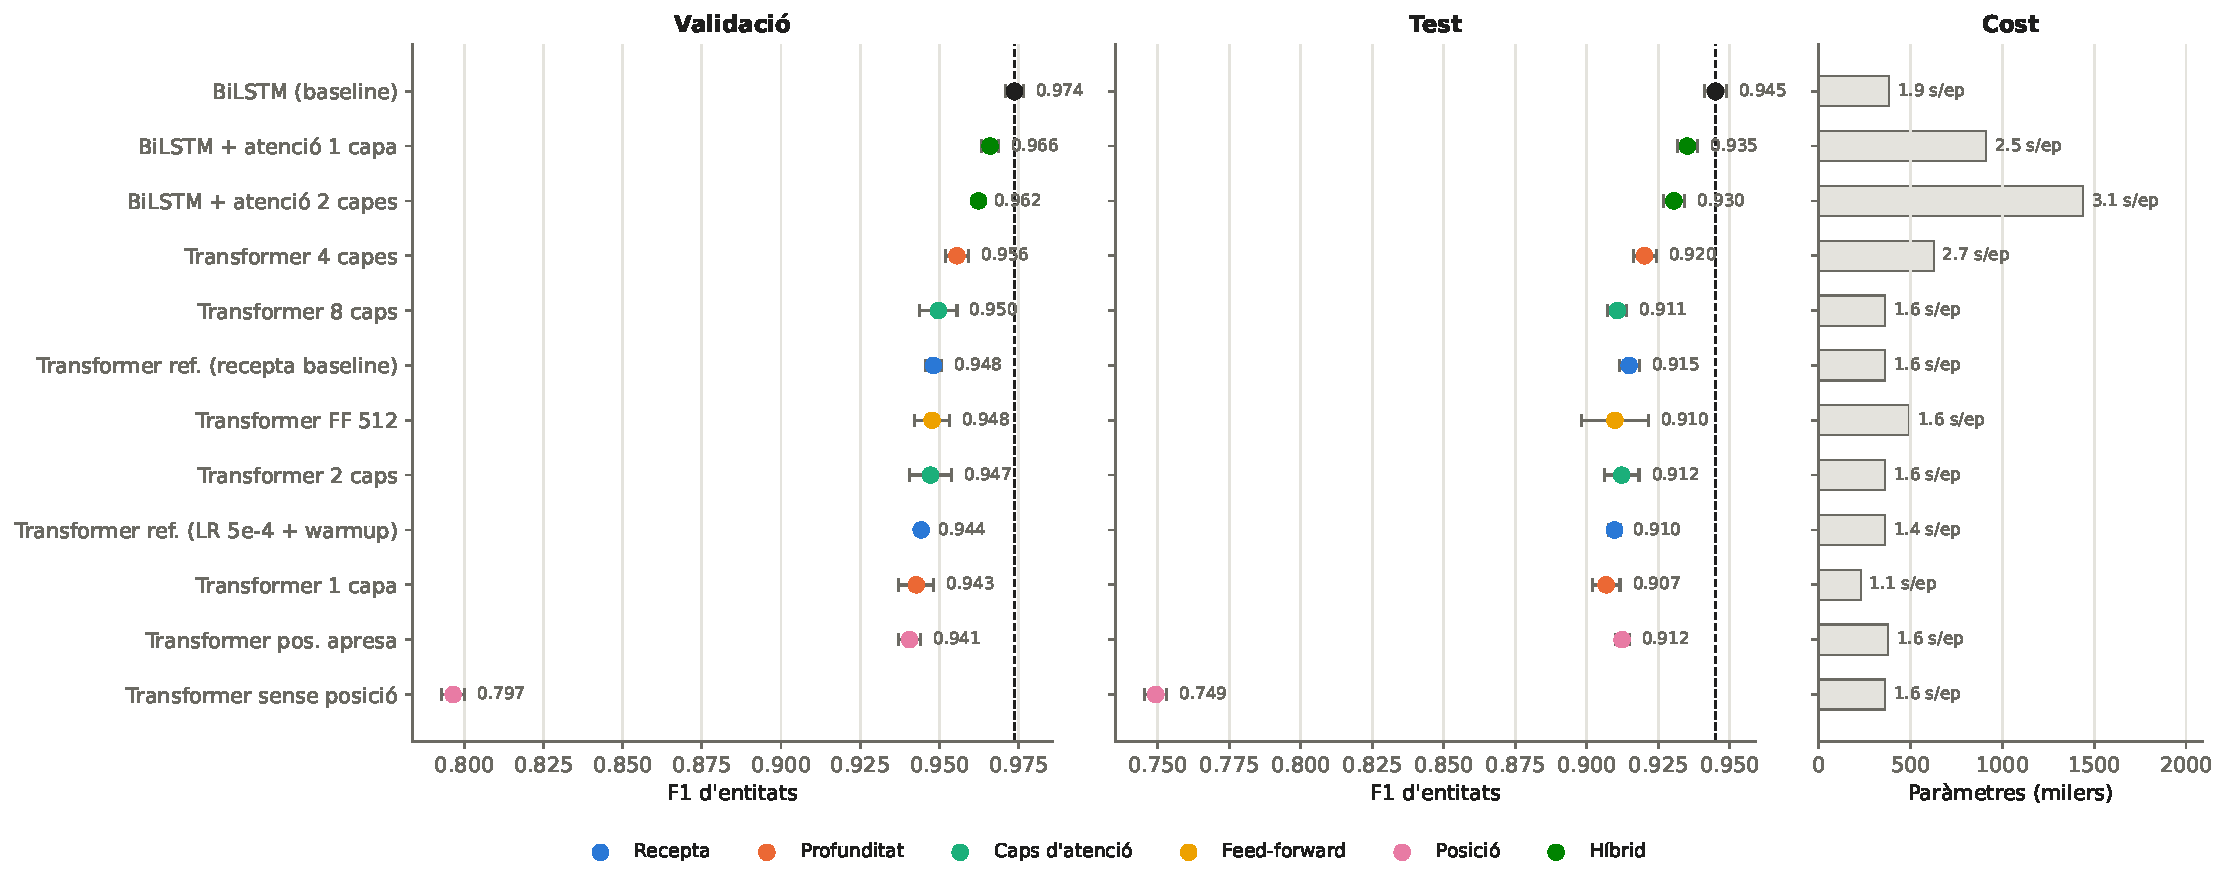
\includegraphics[width=0.9\linewidth]{ex7_4_transformer}
\caption{Variants Transformer i híbrids BiLSTM + atenció: F1 de validació i test i cost.}
\label{fig:transformer}
\end{figure}

El Transformer de referència treu 0,948 de validació i 0,915 de test, tres punts per sota de la BiLSTM, i perd deu
punts de F1 macro. Sense recurrència, el model ha d'aprendre de les dades no només el significat de les paraules
sinó també el seu ordre, i amb 4.000 frases les classes rares no tenen prou exemples per fer-ho
\citep{jurafsky}. El control sense codificació posicional ho mostra bé: la F1 cau fins a 0,797, perquè el model
no té manera de distingir ``from boston to denver'' de ``from denver to boston''. La posició apresa, per la seva
banda, queda una mica per sota de la sinusoidal.

Dos resultats van en contra del que esperàvem. Pensàvem que més capes portarien a sobreajust, però amb quatre capes
el Transformer millora fins a 0,956, el seu millor resultat. I l'híbrid, que havia d'igualar el baseline, es queda
en 0,966. En aquest segon cas, la distància entre la loss de train i la de validació (0,077) és la més gran de tots
els models amb BiLSTM que hem entrenat (la del baseline és de 0,047), i això apunta a sobreajust de les capes
d'atenció, cosa que l'apartat següent confirma.

% ---------------------------------------------------------------------------------------------------------
\subsection{Regularització amb dropout (7.5)}
\label{sec:dropout}

Hem afegit dropout a l'embedding, entre capes recurrents \citep{zaremba}, abans del classificador i dins del
Transformer, en tres models diferents: el baseline, una BiLSTM 2$\times$256 i l'híbrid amb atenció. Primer hem
provat cada posició per separat amb $p=0{,}3$ i després totes juntes amb $p=0{,}1$, $0{,}3$ i $0{,}5$ (a l'híbrid,
només 0,1 i 0,3) (figura~\ref{fig:dropout}).

\begin{figure}[ht]
\centering
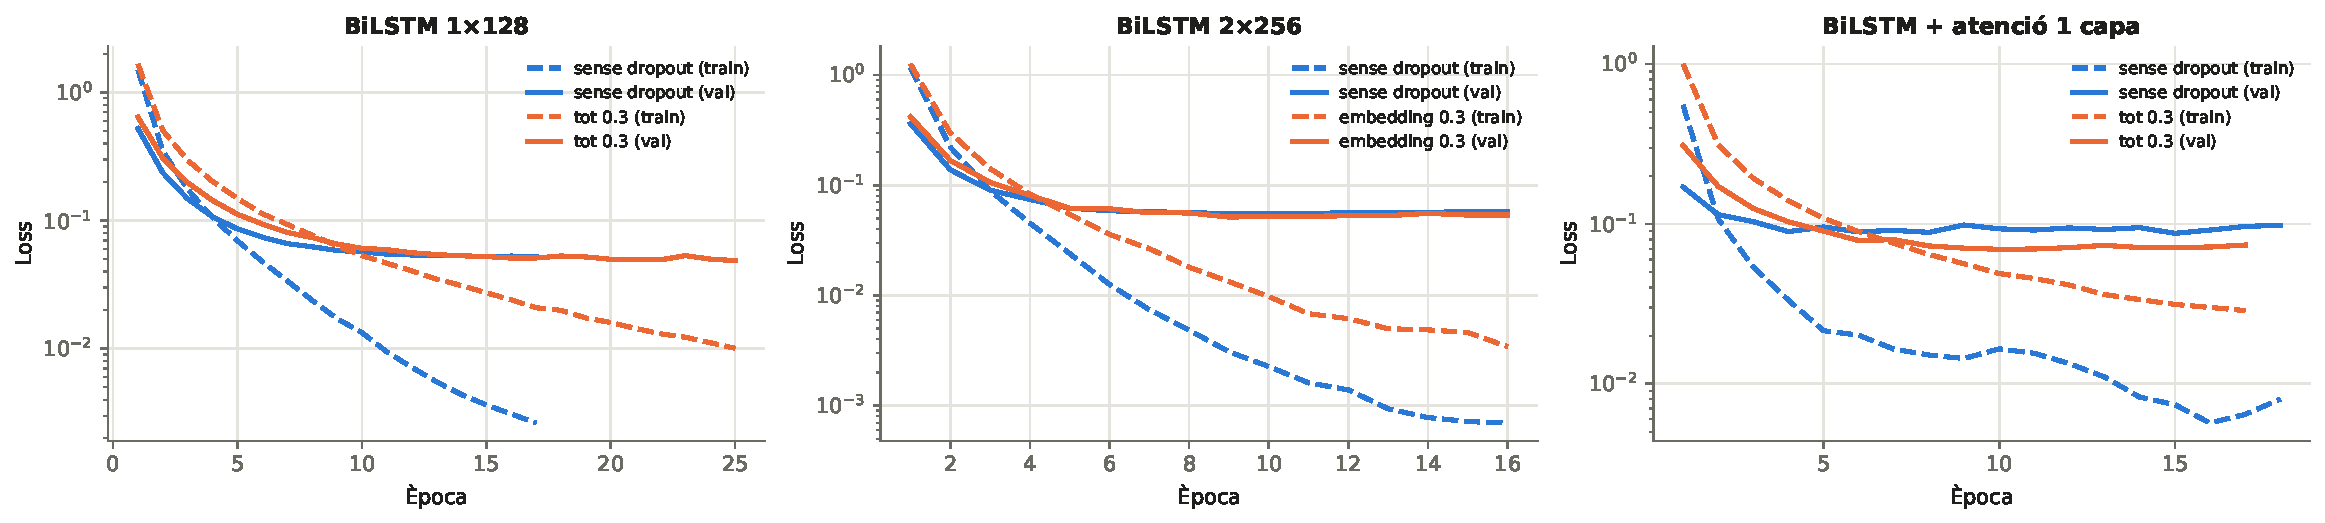
\includegraphics[width=\linewidth]{ex7_5_dropout_curves}
\caption{Loss de train (discontínua) i validació (contínua) sense dropout i amb la millor variant de dropout,
per a cadascun dels tres models.}
\label{fig:dropout}
\end{figure}

Al baseline, un dropout de 0,3 a l'embedding i al classificador millora 0,3 punts de validació, 0,6 de test i tres
de F1 macro, i a test gairebé tota la millora ve del dropout de l'embedding. Té sentit en un vocabulari on moltes
paraules surten poques vegades. Si pugem fins a $p=0{,}5$, la distància entre la loss de train i la de validació
gairebé desapareix, però la F1 torna a baixar.

Per a l'híbrid amb atenció, el dropout és el que el fa funcionar: la F1 passa de 0,966 a 0,974 de validació i de
0,935 a 0,948 de test, i la distància de loss es redueix a la meitat. Tot i així, l'híbrid arriba al nivell del
baseline però no el supera.

La BiLSTM 2$\times$256, en canvi, contradiu la hipòtesi. Era el model amb més paràmetres dels tres i el dropout no
li canvia la F1, tot i que la distància de loss sí que es redueix, de 0,055 a 0,025 amb $p=0{,}5$. Interpretem que
l'aturada ja talla l'entrenament de la BiLSTM abans que el sobreajust arribi a les prediccions, mentre que les
capes d'atenció sobreajusten tan de pressa que l'aturada no hi arriba a temps.

% ---------------------------------------------------------------------------------------------------------
\subsection{Balanceig de les classes (7.6)}
\label{sec:balanceig}

Hem ponderat la cross-entropy segons la freqüència de cada etiqueta amb cinc esquemes: la inversa de la
freqüència i la inversa de l'arrel, totes dues amb i sense límit, i el nombre efectiu de mostres \citep{cui}. També
hem provat de reduir només el pes de \etq{O} (figura~\ref{fig:balanceig}). Els pesos estan normalitzats perquè el
token mitjà pesi 1, i això permet veure fins a quin punt són extrems: amb la inversa pura, una etiqueta vista un sol
cop pesa 260 vegades més que el token mitjà i \etq{O} gairebé no compta.

\begin{figure}[ht]
\centering
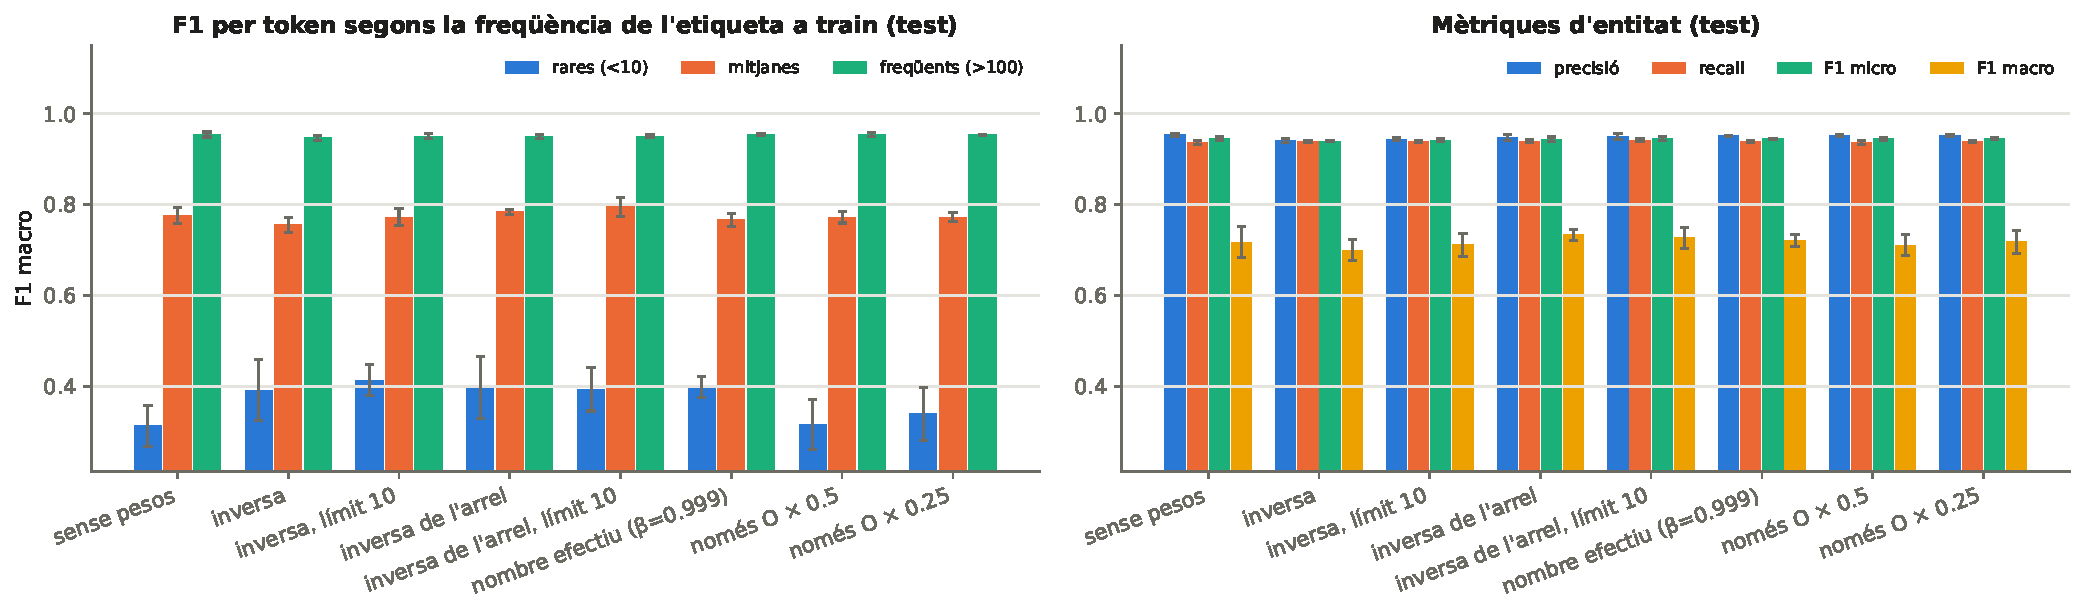
\includegraphics[width=\linewidth]{ex7_6_balanceig}
\caption{Esquemes de pesos de classe. Esquerra: F1 per token segons la freqüència de l'etiqueta a train. Dreta:
precisió, recall i F1 micro i macro d'entitats a test.}
\label{fig:balanceig}
\end{figure}

Les classes rares (menys de 10 exemples a train) són les que més en surten beneficiades: la seva F1 per token passa
de 0,31 a 0,39-0,41 amb qualsevol esquema basat en la freqüència, i la F1 macro per token puja entre un i tres
punts, a canvi de perdre una mica de precisió. La F1 micro d'entitats, però, no millora amb cap esquema, i la
inversa pura fins i tot l'empitjora mig punt, si bé les seves tres llavors arriben al límit de 40 èpoques i el
resultat s'ha de llegir com una cota inferior. L'esquema que dona el millor equilibri és la inversa de l'arrel amb
límit 10, que manté la F1 micro i guanya tres punts de F1 macro per token. Reduir només el pes de \etq{O}, en
canvi, no té cap efecte.

Com que el model final es tria per F1 micro, els pesos no hi entren. Si el sistema hagués de prioritzar les
entitats poc freqüents, la inversa de l'arrel amb límit seria l'opció a triar.

% ---------------------------------------------------------------------------------------------------------
\subsection{Experiments addicionals: CRF, esquema d'etiquetes i vocabulari}
\label{sec:extres}

També hem implementat un CRF lineal \citep{crf}, amb els algorismes forward i Viterbi, i n'hem comprovat el
càlcul enumerant totes les seqüències possibles en un cas petit. L'hem creuat amb l'esquema d'etiquetes en un
disseny 2$\times$2 (taula~\ref{tab:extres}). La F1 d'entitats és comparable entre BIO i BILOU perquè la conversió
no perd informació i les entitats de referència són les mateixes.

\begin{table}[ht]
\centering\small
\caption{Esquema i decodificador (3 llavors). Invàlides: frases de test amb alguna transició impossible, com una
\etq{L-x} sense \etq{B-x} al davant.}
\label{tab:extres}
\begin{tabular}{lccccc}
\toprule
Configuració & Val F1 & Test F1 & F1 macro test & Invàlides (test) & s/època \\
\midrule
BILOU + softmax (baseline) & 0,9737 & 0,9450 & 0,717 & 44 & 1,9 \\
BILOU + CRF                & 0,9742 & 0,9462 & 0,729 & 26 & 7,8 \\
BIO + softmax              & 0,9740 & 0,9446 & 0,727 & 23 & 2,0 \\
BIO + CRF                  & 0,9741 & 0,9460 & 0,737 & 15 & 7,8 \\
$\texttt{min\_freq}=1$     & 0,9739 & 0,9475 & 0,721 & 41 & 2,0 \\
\bottomrule
\end{tabular}
\end{table}

La nostra hipòtesi era que el CRF eliminaria gairebé totes les seqüències invàlides, i les redueix entre un 35 i un
40\%. El motiu és que aprèn les transicions a partir de les dades, sense cap restricció imposada, i les transicions
entre etiquetes rares queden mal estimades; prohibir explícitament les transicions impossibles durant Viterbi les
eliminaria del tot. En F1 micro el CRF no canvia res, millora un punt la F1 macro i multiplica per quatre el temps
per època.

Entre BIO i BILOU no hi ha diferència de F1. BILOU produeix el doble de seqüències invàlides amb softmax, i
l'avantatge d'indicar explícitament el final de cada entitat no compensa passar de 119 a 178 classes. Tampoc no
canvia res fer servir $\texttt{min\_freq}=1$.

% ---------------------------------------------------------------------------------------------------------
\subsection{Model final, ablació i significança}
\label{sec:final}

El model final el construïm automàticament a partir dels resultats de validació: de cada apartat agafem la millor
variant i només l'incorporem si supera la seva referència per més d'una desviació estàndard. Amb aquest criteri hi
han entrat GloVe-300 congelat, la char-CNN i el dropout de 0,3, tot sobre la mateixa BiLSTM d'una capa del
baseline. L'encoder, els pesos de classe i el CRF s'han quedat fora, perquè els seus guanys (+0,27, +0,02 i +0,04
punts) no superen la desviació entre llavors. Per a l'ablació hem reentrenat el model final traient cada component,
aquesta vegada amb cinc llavors (taula~\ref{tab:final}).

\begin{table}[ht]
\centering\small
\caption{Model final, ablació i control sense \mindelta{} (5 llavors). Paràm.: paràmetres entrenables (els
vectors GloVe congelats no hi compten).}
\label{tab:final}
\begin{tabular}{lcccr}
\toprule
Configuració & Val F1 & Test F1 & F1 macro test & Paràm. \\
\midrule
Baseline        & 0,9738 $\pm$ 0,0021 & 0,9463 $\pm$ 0,0035 & 0,727 & 386k \\
\textbf{Model final} & \textbf{0,9789 $\pm$ 0,0016} & \textbf{0,9552 $\pm$ 0,0021} & \textbf{0,777} & 547k \\
final $-$ GloVe    & 0,9792 & 0,9539 & 0,763 & 446k \\
final $-$ char-CNN & 0,9778 & 0,9527 & 0,771 & 486k \\
final $-$ dropout  & 0,9783 & 0,9544 & 0,778 & 547k \\
\midrule
Baseline, sense \mindelta{}    & 0,9760 $\pm$ 0,0026 & 0,9498 $\pm$ 0,0035 & 0,736 & 386k \\
Model final, sense \mindelta{} & 0,9816 $\pm$ 0,0020 & 0,9568 $\pm$ 0,0015 & 0,791 & 547k \\
\bottomrule
\end{tabular}
\end{table}

El model final millora el baseline en 0,9 punts de F1 a test i en cinc de F1 macro (figura~\ref{fig:resum}). Per
saber si aquesta diferència és real o soroll, hem fet un bootstrap pareat sobre les frases de test, llavor a llavor,
i la millora és significativa en les cinc llavors, amb un p-valor unilateral de com a màxim 0,026.

\begin{figure}[ht]
\centering
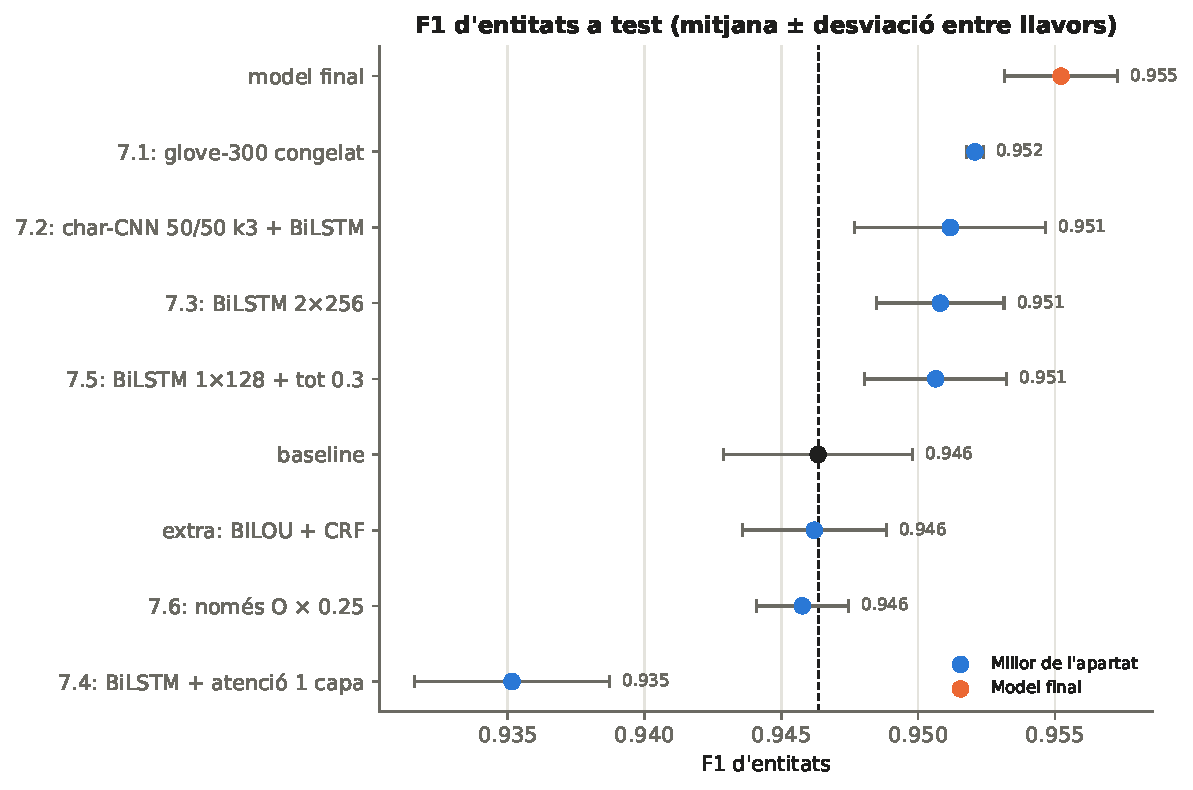
\includegraphics[width=0.65\linewidth]{resum_global}
\caption{F1 d'entitats a test de la millor variant de cada apartat (per validació), del baseline i del model
final (mitjana $\pm$ desviació entre llavors).}
\label{fig:resum}
\end{figure}

L'ablació mostra que els tres components se solapen. El que més pesa és la char-CNN, sense la qual el model perd
0,25 punts de test. Sense GloVe, la validació gairebé no canvia, però el test baixa 0,13 punts i la F1 macro, 1,4.
Treure el dropout queda dins del soroll. Per separat, cadascun millorava el test entre 0,56 i 0,71 punts, i junts
n'aporten 0,9, menys de la meitat de la suma. Com que tots tres milloren la representació de les paraules poc
freqüents, és raonable que en part corregeixin els mateixos errors.

Ens quedava una qüestió per resoldre. El model final convergeix més a poc a poc que el baseline (millor època 16,8
enfront de 12,6), i un criteri d'aturada massa estricte podia estar tallant el baseline abans d'hora i inflant la
diferència. Per comprovar-ho, hem reentrenat tots dos models sense \mindelta, amb paciència 10 i fins a 60 èpoques.
Tots dos milloren i la diferència baixa de 0,89 a 0,70 punts, però continua sent significativa en quatre de les
cinc llavors, la F1 macro hi guanya 5,4 punts i la desviació del model final és menys de la meitat de la del
baseline.

% ---------------------------------------------------------------------------------------------------------
\subsection{Anàlisi d'errors}
\label{sec:errors}

Per acabar, hem classificat cada error d'entitat del test en quatre tipus: tipus equivocat (el tram és correcte
però l'etiqueta no), límits equivocats, entitat no detectada i entitat inventada (taula~\ref{tab:errors}). Per no
quedar-nos amb la llavor més afortunada, fem servir l'execució amb la F1 de validació mediana.

\begin{table}[ht]
\centering\small
\caption{Distribució dels errors d'entitat a test.}
\label{tab:errors}
\begin{tabular}{lcc}
\toprule
Categoria & Baseline & Model final \\
\midrule
Tipus equivocat    & 52\% & 63\% \\
Inventada          & 20\% & 16\% \\
No detectada       & 16\% & 8\% \\
Límits equivocats  & 12\% & 14\% \\
\bottomrule
\end{tabular}
\end{table}

El model final deixa escapar menys entitats, i el que li queda són sobretot errors de tipus. La confusió més
freqüent, en tots dos models, és predir \etq{toloc.city\_name} on l'etiqueta correcta és \etq{city\_name}, i els
exemples n'expliquen el motiu. A ATIS, les ciutats i els estats sense rol apareixen en preguntes que no parlen d'un
trajecte, com ``list california airports'' o ``which airport is closest to ontario california'', però a train
només el 2,4\% de les ciutats no tenen rol i \etq{state\_name} hi surt una sola vegada (al test, nou). Per això
\etq{state\_name} té F1 zero al test i \etq{city\_name} té un recall de 0,54. Encertar aquests casos requereix
saber què demana la frase, que és justament la tasca de la primera part de la pràctica.
